\section{Conclusion}

% \begin{frame}{Open access and education}
%     \vspace{-4em}
%     \begin{itemize}
%         \item Open access: a dedicated portal planned
%         \item Education: \textcolor{blue}{\texttt{astroparticle.online}}
%     \end{itemize}
%     \centering
%     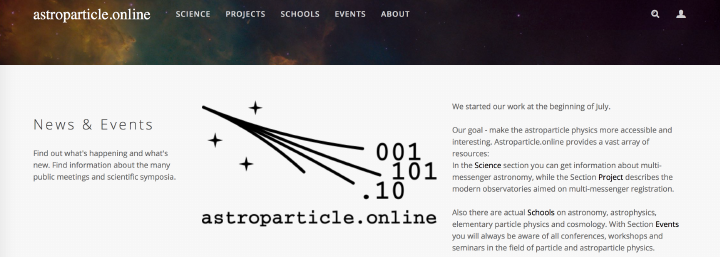
\includegraphics[width=0.85\textwidth]{pics/astro_onl.png}
% \end{frame}

\begin{frame}{Outlook}
% \textcolor{red}{Improve the translation quality!!!}
    \begin{itemize}
%     \item mdl
%     \item kcdc
%     \item Нужны инструменты совместного доступа к данным различных экспериментов и эффективный бережный менеджмент этих больших объемов данных
%     \item Консоциум gradlc предлагает концепцию дата инжиниринга в области астропартикл физикс, основанный на уже kcdc. 
%     \item В данный момент производятся работы по созданию aggregation data server'a и совместному анализу данных из экспериментов kascade и taiga;
% \item Доступ к ресурса проекта на данный момент частично предоставлен через портал astroparticle.online.
      \setlength{\itemsep}{0pt}
%         \item There are no standard solutions so far for careful sharing and managing large data volumes from various APP experiments, but they are in a high demand;
%         \item The Astroparticle Data Life Cycle data ecosystem is in development by participants of GRADLC Consortium, and based on already existing data portal KCDC and a well-known instruments widely used in particle physics;
%         \item The first stage of development includes building aggregation data server and performing the proof-of-principle joint analysis of data from KASCADE and TAIGA experiments are currently being developed;
%         \item Access to the project resource is now partially provided through the astroparticle.online web-portal;
%         \item Most of the data of KASCADE are available on KCDC web-portal: \textcolor{kit-blue70}{https://kcdc.ikp.kit.edu/}
	\item Solutions for careful sharing and managing large data volumes are in a high demand in the field;
        \item The Astroparticle Data Life Cycle data ecosystem is in development by participants of GRADLC Consortium;
        \item It is based on already existing data portal KCDC and a well-known instruments widely used in particle physics;
        \item The development includes building data aggregation and application servers and a proof-of-principle joint analysis of data from KASCADE and TAIGA experiments;
        \item \textbf{The project resources are partially provided in open access for science and education at the \textcolor{kit-blue70}{astroparticle.online} web-portal};
        \item Most of the data of KASCADE are available on KCDC web-portal: \textcolor{kit-blue70}{https://kcdc.ikp.kit.edu/}


    \end{itemize}
\end{frame}

% \subsection{The end}
% \begin{frame}{}
%     \begin{center}
%         \textcolor{kit-green100}{\Huge Thank you\\for your attention!\vspace{1em}}  
%         \Large Any questions?
%     \end{center}
% \end{frame}
